\section{Discussion\label{section:inductive-discussion}}


\subsection{Correctness\label{subsection:inductive-discussion-correctness}}

Proving the correctness of our approach amounts to show that the synthesized system is consistent with the scenarios and domain knowledge taken in input. We discuss proof arguments for the different algorithm settings, starting with the simplest case of RPNI and integrating additional features afterwards, such as scenario questions and consistency with domain knowledge.

Fig.~\ref{synthesis-flow-model} summarizes our approach, which proceeds in two steps: a system LTS is first synthesized, then projected onto agent LTS. In the sequel,
\begin{itemize}
\item $Sc = (S^+,S^-)$ denotes a scenario collection; its positive and negative behaviors are denoted by $\mathcal{L}^+(Sc)$ and $\mathcal{L}^-(Sc)$, respectively.
\item $\mathcal{L}(\mbox{System})$ denotes the behaviors captured by the inferred system LTS.
\item $\mathcal{L}(Ag)$ denotes the behaviors of an arbitrary agent $Ag$.
\item $\mathcal{L}(\agentscomposed)$ denotes the behaviors obtained when individual agent LTS are composed back again.
\end{itemize}

\begin{figure}\centering
\scalebox{.65}{
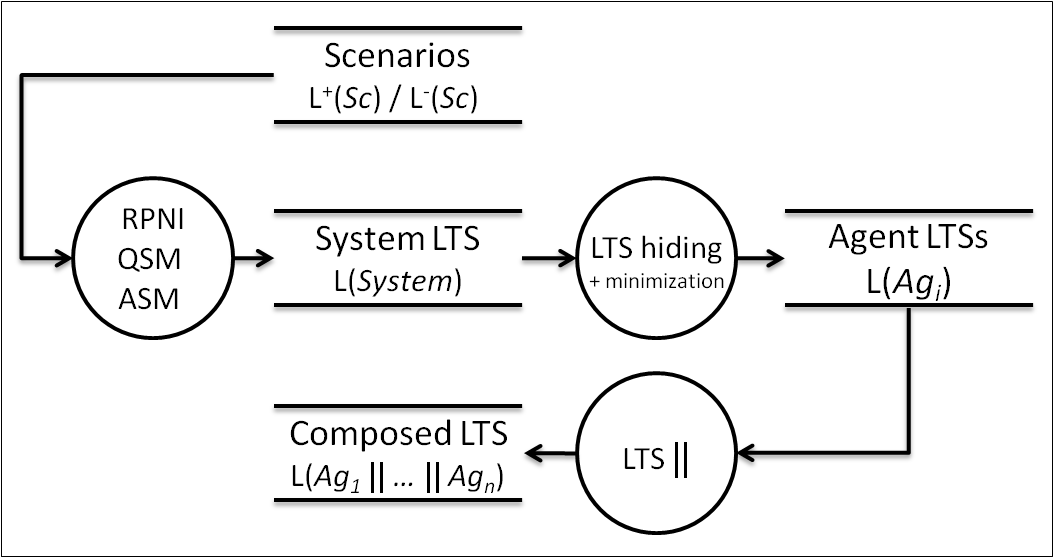
\includegraphics[trim=3mm 3mm 3mm 3mm, clip]{src/4-inductive/images/synthesis-flow-model}}
\caption{Inductive synthesis steps and products.\label{figure:synthesis-flow-model}} 
\end{figure}

Remember from Section~\ref{subsection:inductive-synthesis-statement} that the specification requires three conditions to hold: 
\begin{itemize}
\item The \emph{structural consistency} condition requires scenarios and agent state machines to agree on the respective agent interfaces.
\item The \emph{consistent agent view} condition requires each agent state machine to cover the positive scenario behaviors along the corresponding timeline.
\begin{align}
\mathcal{L}^+(Sc_{\downarrow Ag}) \subseteq \mathcal{L}(Ag)\mbox{~for each agent $Ag$}\label{proof:consistent-agent-view}
\end{align}
where $Sc_{\downarrow Ag}$ denotes the positive behaviors along $Ag$'s timeline in a scenario collection $Sc = (S^+, S^-)$:
\begin{align}
\mathcal{L}^+(Sc_{\downarrow Ag}) = \bigcup_{P \in S^+} \mathcal{L}(P_{\downarrow Ag})~~\cup~~\bigcup_{N \in S^{-}} \mathcal{L}^{+}(N_{\downarrow Ag})\label{proof:lemma-sc-projection}
\end{align}

This is a a slight generalization of the concept of agent traces along a single scenario timeline $M_{\downarrow Ag}$, introduced in Section~\ref{section:background-scenarios}. Observe, however, that it takes both positive and negative scenarios into account.
\item The \emph{consistent system view} requires the system to cover all positive scenarios and reject all negative ones. 
\begin{align}
&\mathcal{L}^+(Sc) \subseteq \mathcal{L}(\agentscomposed)\label{proof:consistent-system-view-1}\\
&\mathcal{L}^-(Sc) \cap      \mathcal{L}(\agentscomposed) = \emptyset\label{proof:consistent-system-view-2}
\end{align}
\end{itemize}

\subsubsection*{Structural consistency and consistent agent view}

Provided the \emph{consistent system view} holds, the decomposition step guarantees that the \emph{structural consistency} and \emph{consistent agent view} conditions hold as well. In particular, for each agent $Ag$, (\ref{proof:consistent-agent-view}) can be derived from (\ref{proof:consistent-system-view-1}) using the following relations:
\begin{align}
&\mathcal{L}(X) \subseteq \mathcal{L}(Y) \implies \mathcal{L}(X) \setminus I \subseteq \mathcal{L}(Y) \setminus I\label{proof-agent-consistency-2}\\
&\mathcal{L}^+(Sc) \setminus \Sigma_{Ag}^c \subseteq \mathcal{L}(\agentscomposed) \setminus \Sigma_{Ag}^c\label{proof-agent-consistency-3}\\
&\mathcal{L}^+(Sc) \setminus \Sigma_{Ag}^c = \mathcal{L}^+(Sc_{\downarrow Ag})\label{proof-agent-consistency-4}\\
&\mathcal{L}(\agentscomposed) \setminus \Sigma_{Ag}^c = \mathcal{L}(Ag)\label{proof-agent-consistency-5}
\end{align}
where $\Sigma_{Ag}^c$ denotes the set of all system events excluding those of $Ag$'s interface.

(\ref{proof-agent-consistency-2}) states that behavior inclusion is preserved under hiding (see Section~\ref{subsection:lts-hiding}). 
Therefore, (\ref{proof:consistent-system-view-1}) can be rewritten as (\ref{proof-agent-consistency-3}). 
(\ref{proof-agent-consistency-4}) can be derived from (\ref{proof:lemma-sc-projection}) and the definition of $M_{\downarrow Ag}$ (see Section~\ref{subsection:background-positive-scenarios}). 
(\ref{proof-agent-consistency-5}) follows from material on LTS in Section~\ref{section:background-state-machines}. 
(\ref{proof:consistent-agent-view}) is derived by rewriting (\ref{proof-agent-consistency-3}) thanks to (\ref{proof-agent-consistency-4}) and (\ref{proof-agent-consistency-5}).

\subsubsection*{Consistent system view}

Condition (\ref{proof:consistent-system-view-1}) follows from two main properties of our approach:
\begin{itemize}
\item The synthesized system LTS covers all positive scenario behaviors, as guaranteed by RPNI itself:
\begin{align}
&\mathcal{L}^+(Sc) \subseteq \mathcal{L}(\mbox{System})\label{proof:consistent-system-view-d-1}
\end{align}
A proof of RPNI convergence is presented in~\cite{Oncina:1993} in the more general case of transducer learning. 
\item Projecting the system LTS on agent alphabets and recomposing their LTS afterwards cannot restrict behaviors:
\begin{align}
&\mathcal{L}(Ag_i) = \mathcal{L}(\mbox{System}) \setminus \Sigma_{Ag_i}^c\label{proof:consistent-system-view-d-2}\\
&\mathcal{L}(\mbox{System}) \subseteq \mathcal{L}(\agentscomposed)\label{proof:consistent-system-view-d-3}
\end{align}
(\ref{proof:consistent-system-view-d-2}) follows from (\ref{definition:decomposition-step}) that defines the LTS operation applied for the decomposition step (see Section~\ref{subsection:inductive-synthesis-approach}). (\ref{proof:consistent-system-view-d-3}) can be derived from properties of LTS hiding and composition operators (see Section~\ref{section:background-state-machines}).
\end{itemize} 

Condition (\ref{proof:consistent-system-view-2}) requires the composed system to exclude all negative scenarios. Our approach only guarantees a weaker condition, namely,
\begin{align*}
&\mathcal{L}^-(Sc) \cap \mathcal{L}(\mbox{System}) = \emptyset
\end{align*}

In other words, the induction algorithm ensures that the \emph{system LTS} excludes all negative scenarios~\cite{Oncina:1993}. This property can however be lost after the decomposition and recomposition steps, as explained now.

\subsubsection*{Implied scenarios}

The reason has to be found in the possible occurence of so-called \emph{implied scenarios}. Remember from Section~\ref{subsection:background-hmsc} that implied scenarios may appear when a system is specified globally while implemented component-wise ~\cite{Alur:2000, Uchitel:2004}. In our case, the set of implied scenarios is precisely captured by:
\begin{align*}
\mathcal{L}(\agentscomposed) \setminus \mathcal{L}(\mbox{System})
\end{align*}

In other words, implied scenarios are system behaviors that the system LTS does not accept but which necessarily appear when composing the agent LTSs. Implied scenarios appear because, once distributed, the agents lack monitoring abilities to restrict their behavior so as to precisely match the system LTS.

Not all implied scenarios are problematic in practice. In particular, it might happen that all implied scenarios denote examples of desired behaviors. In that case, the presence of implied scenarios is not problematic and may be seen as the result of a second generalization step due to the decomposition and recomposition of agent LTS. The second generalization step proves useful as a structurally complete scenario collection might be difficult to obtain in the first place (see later).

Negative implied scenarios, that is, counterexamples of desired behaviors, are more problematic. In particular, a behavior trace $t$ could be such that the following conditions hold:
\begin{align}
&t \in \mathcal{L}^-(Sc)\\
&t \notin \mathcal{L}(\mbox{System})\\
&t \in \mathcal{L}(\agentscomposed)
\end{align}
that is, (a) $t$ denotes a system behavior explicitly rejected through a negative scenario; it might be a question answered negatively; (b) $t$ is correctly rejected by the system LTS; (c) $t$ is still be exhibited by the composed system.

In such case, observe that the condition (\ref{proof:consistent-system-view-2}) does not hold. In other words, our approach fails to guarantee a consistent system view between scenarios and state machines in presence of negative implied scenarios.

As with other scenario approaches, e.g. \cite{Alur:2000, Uchitel:2004}, fixing the presence of negative implied scenarios requires rethinking the agent decomposition and their interfaces. The root cause of implied scenarios problems has to be found in the structural decomposition of the system, not in the particular technique used to infer state machines from scenarios.

\subsubsection*{Correctness in the presence of scenario questions}

The specification of QSM has been strengthened in Section~\ref{section:lts-induction-from-mscs}. This strengthening required the synthesized system to be consistent with all scenario questions in addition to the initial scenario collection. 

Arguments about the \emph{structural consistency} and \emph{consistent agent view} conditions remain unchanged. The same applies for implied scenarios so that we only prove the consistency of the system LTS induced by QSM.

This can be proven by induction along as follows:
\begin{itemize}
\item The base case captures a QSM run where all scenario questions are answered positively. In such case, QSM roughly reduces to RPNI, for which the following conditions are known to hold \cite{Oncina:1993}:
\begin{align}
&\mathcal{L}^+(Sc) \subseteq \mathcal{L}(\mbox{System})\\
&\mathcal{L}^-(Sc) \cap \mathcal{L}(\mbox{System}) = \emptyset
\end{align}

For this particular QSM run, we still need to prove that all accepted scenario questions are accepted by the system LTS. Observe that when accepted (line 7 in Algo.~\ref{QSM}), these scenarios are consistent with the current solution $A_{new}$ (see line 4). The system LTS returned by QSM is a quotient automaton of $A_{new}$; Definition \ref{definition:quotient-automaton} ensures that the system LTS accepts those scenarios as well.
\item Every time a scenario question is rejected by the oracle, the scenario collection is correctly extended (see line 9). Provided the oracle does not make classification errors, as required in preconditions, the scenario collection remains consistent. The recursive call on the extended scenario collection provides the inductive step (see line 10).
\end{itemize}

\subsubsection*{Domain Knowledge}

\subsubsection*{Control information}

\subsection{Rationale behind the generalization step}

Our synthesis requirements include ``behavior generalization''. Looking at relation (\ref{relation:inductive-language-refinements}) we might ask ourselves what drives the generalization process and until when. By construction, the first automaton $A_0$ already meets the consistent system view conditions (\ref{relation:inductive-invariant}) and (\ref{relation:inductive-invariant-II}). Therefore, $A_0$ is a valid, yet trivial, solution. Why not simply use it?

The answer is to be found in the Occam's principle stating that ``among all models explaining the world equally well, the simplest should be preferred''. Using grammar induction this amounts to searching for the \emph{smallest} automaton consistent with the positive and negative scenarios, also called the \emph{input sample}. The initial automaton $A_0$ is rarely the simplest model according to this criteria. 

Looking for the smallest automaton consistent with an input sample is known to be NP-hard \cite{Gold:1978, Angluin:1978}. The RPNI algorithm offers a consistent approximated solution in polynomial time; this solution is the smallest consistent deterministic automaton when the input sample is rich enough, in particular when it forms a so-called \emph{characteristic sample} (see later) \cite{Oncina:1992}.

\subsection{Future directions}

From a grammar induction point of view, the ASM algorithm can be seen as generalizing any positive regular language $\mathcal{L}^+$ under the control of a negative sample $S^-$. As such, RPNI is thus a special case where the positive language forms a sample $S^+$, that is a finite set of strings.

Moreover, goals and domain properties can still be used to prune the ASM search space with the technique discussed in Section~\ref{subsection:induction-pruning-with-goals}. As goals actually capture negative languages through their tester automaton, this amounts to consider a generalization of ASM to generalize a positive language $\mathcal{L}^+$ under the control of a negative one $\mathcal{L}^-$. This generalization is called ASM$^*$ and briefly discussed in \cite{Lambeau:2008}.
